\chapter{Introducción}
	\label{introduccion}

	Los dispositivos reconfigurables han transitado de módulos de interconexión entre miembros de un sistema electrónico(\textit{glue logic}) ha receptáculos para la integración de sistemas digitales complejos bajo un empaquetado único. El éxito de estos dispositivos se deriva de su capacidad para la implementación de múltiples unidades funcionales con ejecución paralela de tareas.

	El incremento en la cantidad de elementos programables, así como la integración de bloques dedicados a tareas específicas como: bloques para el procesamiento de señales (\textit{DSP}), unidades de aritmética de punto flotante, procesadores de propósito general y bloques de memoria, han abonado para convertir a los dispositivos reconfigurables en plataformas atractivas para la implementación de aceleradores en hardware. El espacio de diseño para aceleradores en hardware reconfigurable ha sido fuertemente influenciado por las arquitecturas desarrolladas para tecnologías de fabricación de circuitos integrados de propósito específico, las cuales, no generan los mismos rendimientos al ser portadas a lógica reconfigurable.

	El resto del capítulo se desenvuelve en el siguiente orden: en la sección \ref{objetivos} se formalizan los objetivos de esta tesis. La sección \ref{motivación} enumera áreas de oportunidad para el sistema desarrollado en este trabajo de investigación. Dentro de la sección \ref{desafíos} se enumera algunos de los retos que se abordaron durante el desarrollo de la tesis. La sección \ref{contribuciones} enumera las principales contribuciones obtenidas como resultado de este trabajo. En la sección \ref{estructura} se ofrece un desglose de la organización del contenido del presente documento. Finalmente, la sección \ref{publicaciones} ofrece un listado de las publicaciones producto del desarrollo de este trabajo.


\section{Objetivos}
	\label{objetivos}
	
	El presente trabajo explora el espacio de diseño de aceleradores de procesamiento interconectados mediante redes en-chip para dispositivos reconfigurables. De manera especifica, el trabajo busca proponer una plataforma para aceleradores en hardware reconfigurable que explote de manera eficiente los recursos y restricciones propios de esta tecnología.

	\subsection{Objetivos particulares}
		\label{objetivos_particulares}
		De manera particular, la arquitectura descrita en este trabajo busca incursionar en los siguientes puntos de diseño:

		\begin{itemize}

			\item 	Diseño de una estructura de interconexión con baja demanda de elementos lógicos para su implementación. Las decisiones de diseño son orientadas por las restricciones de colocación de recursos dentro del dispositivo reconfigurable.

			\item 	Diseño de una interfaz para el intercambio de información entre núcleos de procesamiento y medio de comunicación. El modulo de acoplamiento debe de ocultar los detalles del protocolo de red a las unidades funcionales del sistema.

			\item 	Desarrollo de una estrategia de distribución de carga de trabajo entre núcleos. El modelo de trafico debe de tomar en cuenta las restricciones de área de la tecnología destino, optando por mecanismos eficientes respecto a área para el calculo de trayectoria de paquetes de información a través de la infraestructura de interconexión.  

			\item 	Propuesta de un modelo de interacción entre un acelerador y generadores de datos a procesar.

		\end{itemize}


\section{Motivación}
	\label{motivacion}

	El proceso de investigación llevado a cabo para el desarrollo de esta tesis está motivado de manera principal por aplicaciones que pueden descomponer su operación en unidades homogéneas e independientes de procesamiento.

	\begin{itemize}

			\item 	\textsc{Estimación de movimiento - Block Matching}\cite{chapter0:6701287}: Los algoritmos de estimación de movimiento basados en cotejo de bloques tienen como objetivo el localizar correspondencias de \textit{macro bloques} entre diferentes cuadros de una secuencia de video. La aparición entre cuadros de un patrón representativo de un objeto permite obtener un estimado de la dirección y velocidad de desplazamiento de este mismo. Además, la información proporcionada por el algoritmo puede ser utilizada para la detección de información redundante en la secuencia de video para facilitar el proceso de compresión de la fuente.

			Block matching consiste en 3 pasos fundamentales: en primer lugar el cuadro de la secuencia de video se divide en macro bloques de tamaño constante. A continuación se delimita una región de búsqueda, donde el algoritmo llevará a cabo el proceso de comparación de macro bloques. Finalmente, se procede a la búsqueda de correspondencias de bloques entre cuadros. El flujo de procesamiento se muestra en la figura \ref{fig:ch0_block_matching}. La operación de comparación entre bloques resulta particularmente demandante en casos donde las regiones de búsqueda son amplias o cuando se debe de llevar a cabo el seguimiento de múltiples objetos en cada cuadro de video.

				\begin{figure}
					\begin{center}
						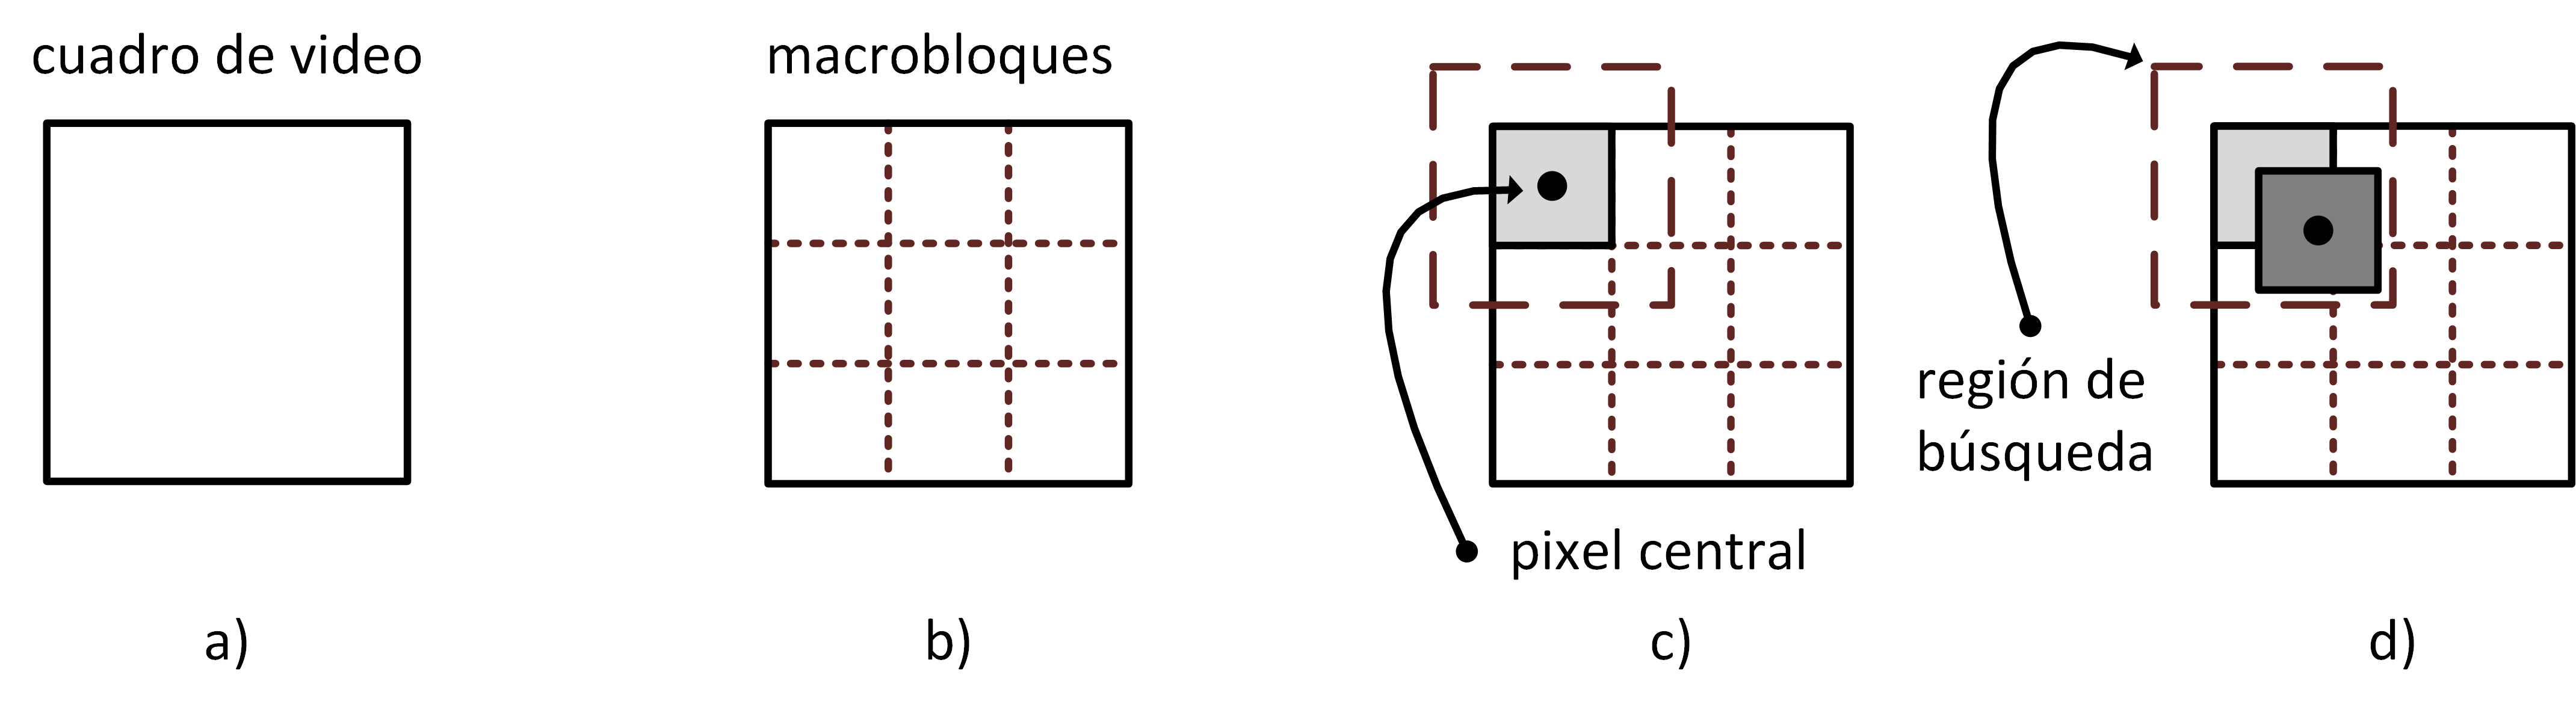
\includegraphics[scale = 0.8]{figures/ch0_block_matching.png}
					\end{center}
					\caption
						{	
							Secuencia simplificada de operación de un algoritmo \textit{block matching}. a) La unidad básica de información es un cuadro de una secuencia de video. b) Los cuadros se dividen en macro bloques de dimensiones constantes. c) El macro bloque se especifica solo con el pixel central y la distancia al límite del bloque. Los macro bloques con información relevante son almacenados para la búsqueda de coincidencias en cuadros posteriores. d) Se inicia la búsqueda del macro bloque en cuadros posteriores de la secuencia de video. La búsqueda se limita a un área especifica denominada región de interés.
						}
					\label{fig:ch0_block_matching}
				\end{figure}


			\item 	\textsc{Redes Neuronales Convolucionales para el procesamiento de imágenes}\cite{chapter0:Ciresan:2011:FHP:2283516.2283603}: Esta clasificación de redes neuronales sigue el esquema de procesamiento denominado \textit{propagación hacia adelante}. El arreglo de neuronas que conforma la red se distribuye en forma de una malla que se sobrepone al campo visual de la aplicación. Su funcionamiento está inspirado en un modelo biológico de procesamiento de imágenes, por lo que sus aplicaciones más comunes es el reconocimiento de patrones.

			Una red neuronal convolucional es un arreglo jerárquico compuesto por capas de neuronas que efectúan tres operaciones: convolución para la extracción de características de alto nivel, capas de sub muestreo para la extracción de patrones de interés, y una capa con conexión completa para la clasificación del objeto alimentado a la red. Las diferentes capas de una red convolucional operan de manera similar a las células simples y complejas que se encuentran el la capa 1 del córtex visual\cite{chapter0:TJP:TJP19591483574}. El esquema de conexión entre capas de convolución y capas de sub muestreo, así como el tipo de entrenamiento para la red, son características que distinguen diferentes implementaciones de este tipo de sistemas. La figura \ref{fig:ch0_convolutional_networks} muestra el modelo general de una red neuronal convolucional.

			\begin{figure}
					\begin{center}
						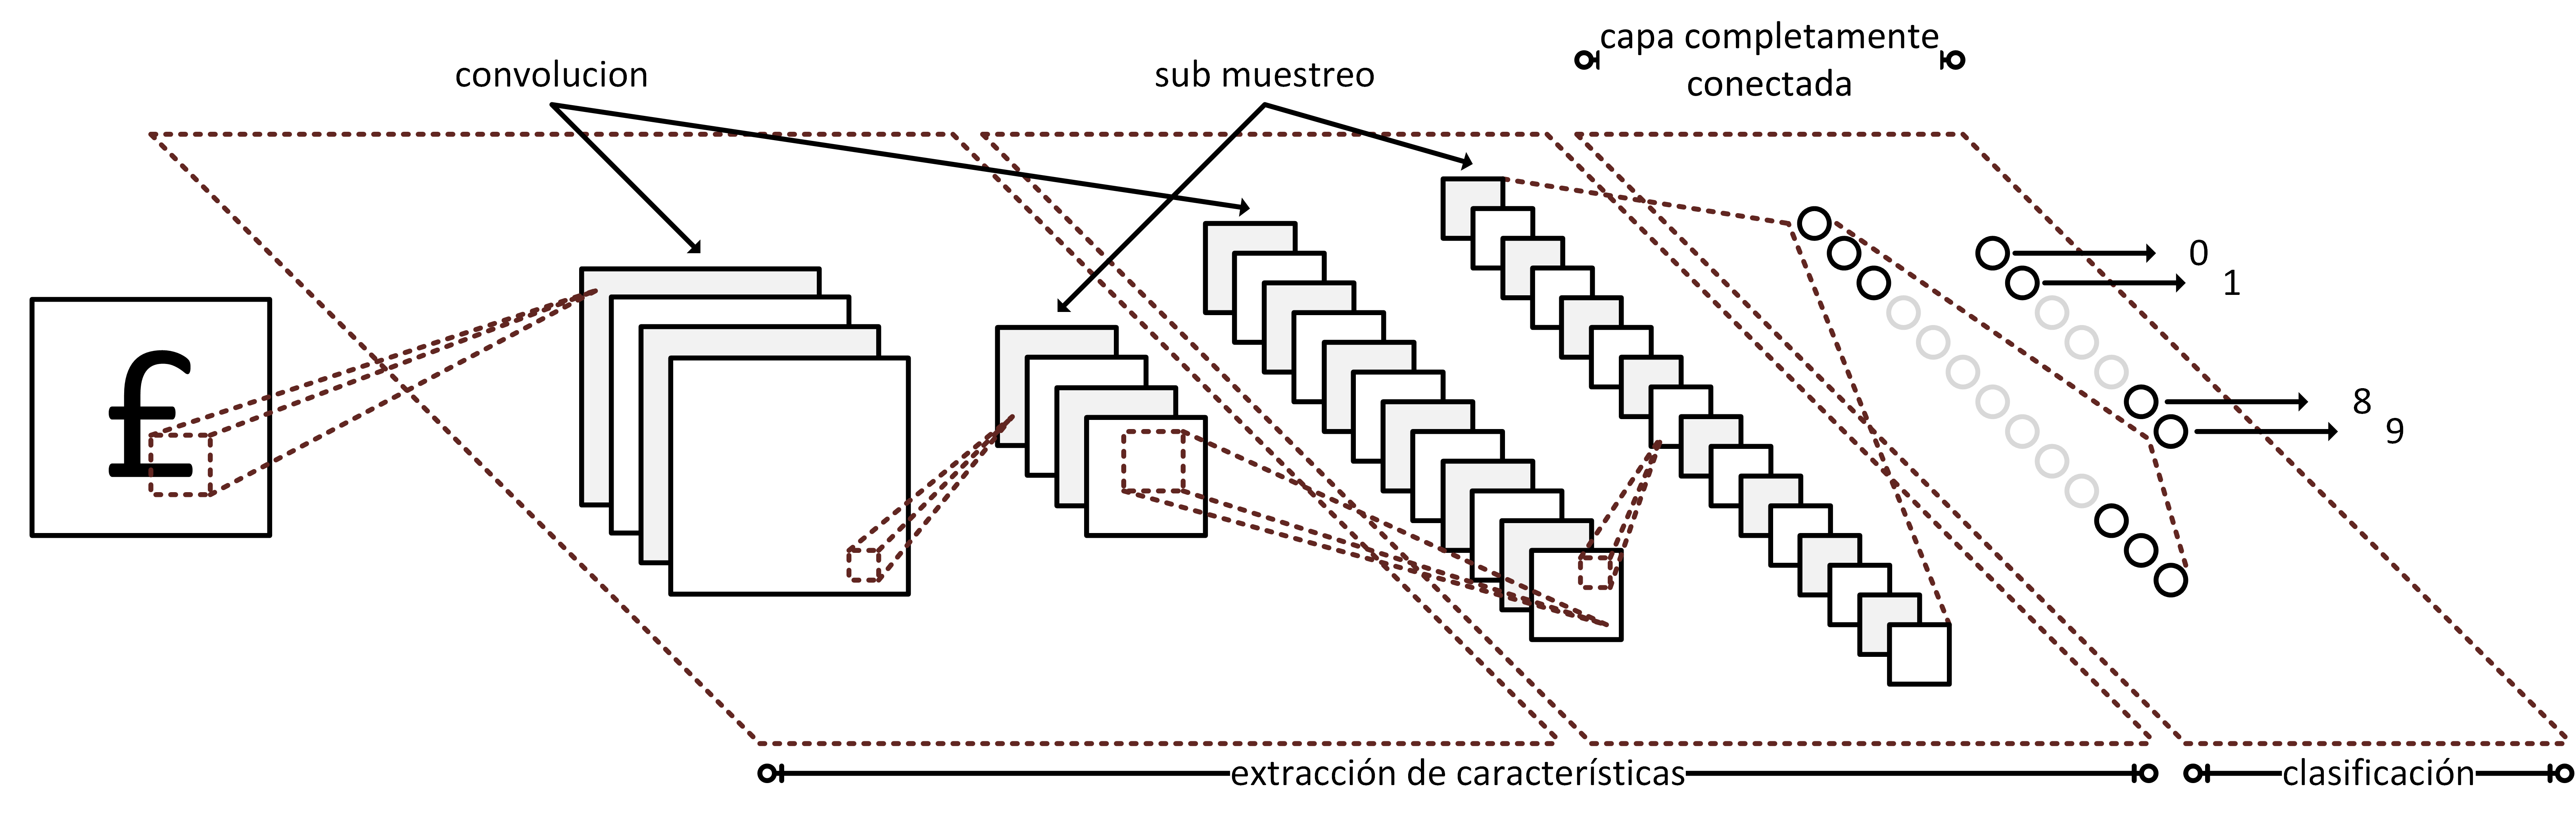
\includegraphics[scale = 0.5]{figures/ch0_convolutional_networks.png}
					\end{center}
					\caption
						{	
							Estructura general de una red neuronal convolucional. El número de capas de convolución/submuestreo determinan la complejidad de los patrones a discernir. El resultado del procesamiento llevado a cabo por la red es la clasificación del patron de entrada a una de las categorías definidas durante el entrenamiento de la red neuronal.
						}
					\label{fig:ch0_convolutional_networks}
				\end{figure}


			\item 	\textsc{Procesamiento de imágenes - Kernels}: En el contexto de procesamiento de imágenes, un kernel o máscara, es una matriz que permite la aplicación de operaciones como: desdibujado, definición, realce, detección de bordes, entre otras. El uso de kernels implica la ejecución de una operación de convolución entre la máscara y un área de la imagen de entrada. La operación de convolución se denota con el operador de multiplicación, sin embargo la operación no es equivalente  al producto de ambos bloques de información, sino a la operación definida en la ecuación \ref{equ:ch0_kernel}.

			\begin{equation}
				\begin{bmatrix}
						a & b & c\\
						d & e & f\\
						g & h & i
				\end{bmatrix}
						\times
				\begin{bmatrix}
						1 & 2 & 3\\
						4 & 5 & 6\\
						7 & 8 & 9
				\end{bmatrix}
				= (1*a) + (2*b) + (3*c) + (4*d) + (5*e) +
				(6*f) + (7*g) + (8*h) + (9*i)
				\label{equ:ch0_kernel}
			\end{equation}

			\begin{figure}
				\captionsetup{singlelinecheck=off}
				\begin{center}
						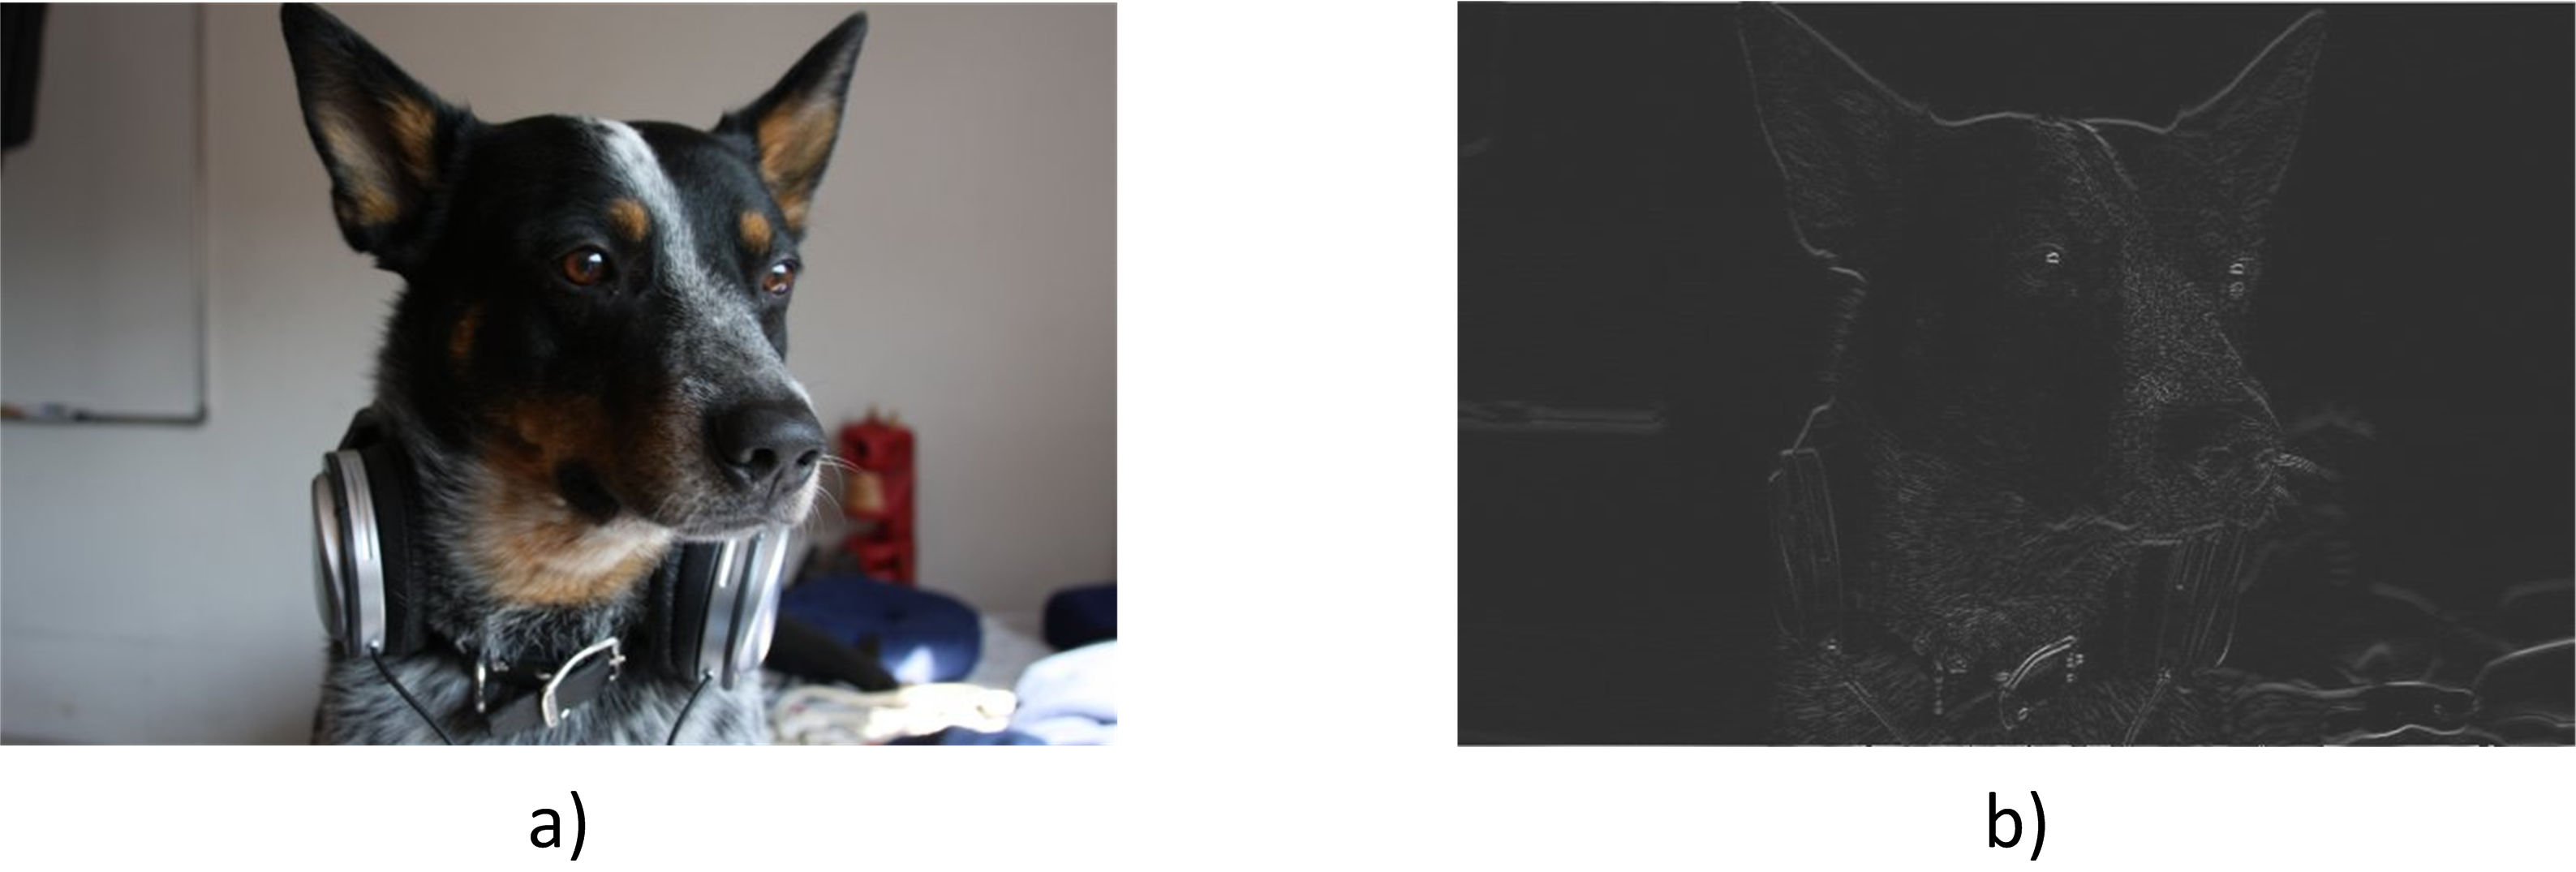
\includegraphics[scale = 0.9]{figures/ch0_kernel_border.png}
				\end{center}
					\caption
						{	
							Detección de bordes en orientación vertical. a) muestra una imagen previa a la aplicación de un kernel de procesamiento. b) presenta el resultado de la aplicación del kernel $\left(\protect\begin{smallmatrix}1\\-1\protect\end{smallmatrix}\right)$
						}
					\label{fig:ch0_kernel_border}
				\end{figure}


			\item 	\textsc{Cifrado - Encriptadores por bloques}: Un encriptador por bloques es la implementación de un algoritmo determinístico que opera sobre conjuntos de bits de dimensiones constantes denominados bloques. Esta familia de encriptadores trabaja con llaves simétricas, en otras palabras utiliza la misma contraseña para el cifrado/descifrado de datos. La teoría detrás de este tipo de encriptadores fue presentada por Claude Shannon\cite{chapter0:6769090} en 1949.

			Los cifradores por bloques llevan a cabo su operación a lo largo de múltiples rondas, las cuales consta de una combinación de operaciones simples como sustituciones y permutaciones. Cada ronda de encriptación utiliza llave derivadas de la llave original, las cuales también son calculadas ronda a ronda.

			Los algoritmos DES\cite{chapter0:NIST:1977:DES}(\textit{Data Encryption Standard}) y AES\cite{chapter0:Daemen:2002:DR:560131}(\textit{Advanced Encryption Standard}) son dos ejemplos populares de esta familia de encriptadores.

		\end{itemize}



\section{Desafíos}
	\label{desafios}

	El diseño de aceleradores en hardware reconfigurable ha evolucionado con el desarrollo de de nuevos métodos de fabricación y nuevas arquitecturas para los dispositivos, sin embargo cada nueva generación de hardware plantea nuevos desafíos para obtener un mejor rendimiento.

	\begin{itemize}

			\item 	\textsc{Restricciones por arquitectura de hardware}: Un conjunto de recursos predefinidos así como una estructura estática, pero abundante de elementos de interconexión, hacen del diseño de circuitos digitales para dispositivos reconfigurables un área de trabajo distinta al diseño tradicional para dispositivos de propósito específico. Este documento se centra en dispositivos reconfigurables FPGA(\textit{Field Programmable Gate Array}).

			Un diseño en hardware reconfigurable debe de tomar en cuenta desde su inicio la organización de recursos internos del dispositivo. Por ejemplo, la arquitectura ASMBL\cite{chapter0:Xilinx:UG474} (\textit{Advanced Silicon Modular Block}) de Xilinx organiza los recursos internos del FPGA en columnas. La distribución de recursos crea una restricción positiva a nivel local, ya que unidades funcionales de un sistema tienen concentrados en un vecindario recursos necesarios para su tendido, entre estos recursos se pueden enumerar: elementos de memoria, multiplicadores, LUTs (\textit{Lookup Table}), árboles de distribución de reloj, etc... Desde el punto de vista de sistema, la restricción resulta desafiante durante el proceso de cierre de tiempos, ya que si dos unidades funcionales del diseño requieren los mismo recursos, una de ellas deberá desplazarse a otra región del dispositivo creando caminos de propagación más largos afectando la frecuencia de operación de todo el diseño. No solo la velocidad del sistema se ve afectada, una planeación pobre durante el inicio del flujo de diseño puede derivar en la pelea por recursos entre unidades, por ejemplo, una unidad funcional puede estar acaparando todo los bloques de memoria embebida de una región obligando a una estructura de interconexión a asentarse en una región remota del dispositivo o simplemente a no poder ser colocada por falta de recursos.

			La diferencia estructural entre dispositivos de diferentes fabricantes acentúa este problema, ya que las primitivas específicas de un dispositivo no son portables entre miembros de distintas familias y entre distintos fabricantes.


			\item 	\textsc{Interconexión de unidades funcionales:} Uno de los paradigmas comunes para la construcción de aceleradores consiste en la generación de múltiples unidades funcionales para ejecutar de manera distribuida una tarea. El principal problema con este acercamiento radica en la distribución de la información a ser procesada entre todos los núcleos de ejecución. El uso de estructuras tipo bus ha sido reemplazado por el uso de redes en-chip\cite{chapter0:976921, chapter0:1511986, chapter0:1347918}, las cuales representan la adaptación del concepto de comunicaciones entre computadoras en una red de área local aplicado a la transmisión de información entre unidades funcionales de un sistema digital en un solo encapsulado.

			Las redes en-chip permiten el transporte información a través de un medio de comunicación distribuido, y se presentan como uno de los candidatos para convertirse en el medio de interconexión estándar para diseños formados por múltiples elementos de procesamiento. Gran parte de los esfuerzos en esta área están enfocados en el desarrollo de mecanismo para proporcionar transacciones de información seguras entre miembros de la red, sin embargo, los mecanismos para proveer un mayor grado de calidad en el servicio de transporte de datos trae consigo un mayor consumo de recursos, al mismo tiempo que agregan latencia derivada los servicios anteriormente referidos.

			\item 	\textsc{Re usabilidad:} El concepto de reutilizar bloques funcionales, comúnmente denominados IP (\textit{Intellectual Property}), es una práctica común el desarrollo de sistemas digitales en FPGAs. Un bloque re utilizable presenta una interfaz  definida de entradas y salidas, así como registros de configuración para facilitar su integración en nuevos diseños. Cuando se trata de bloques que interactúan con un medio de comunicación, se requiere el uso de módulos dedicados al manejo del protocolo de transmisión de datos implementado por el medio.

			El uso de protocolos complejos conlleva al incremento en los recursos necesarios para implementar la lógica de manejo de protocolo, penalizando la latencia de transmisión de un mensaje con los tiempos necesarios para la decodificación de la información de transporte.

			\item \textsc{Hardware reconfigurable no es ASIC:} Gran parte de las arquitecturas de aceleradores en hardware reconfigurable se encuentran fuertemente influenciados por las reglas de diseño establecidas para circuitos de aplicación específica, las cuales no toman en cuenta las restricciones que un diseño reconfigurable afronta. La extrapolación de arquitecturas exitosas en diseños de aplicación específica no siempre producen los mismo resultados en su contraparte reconfigurable.

			El desarrollo de sistemas con múltiples núcleos de procesamiento de propósito general formados con \textit{núcleos-suaves}\cite{chapter0:Microblaze:Xilinx, chapter0:NiosII:Altera} (\textit{Softcores}) es un ejemplo de la degradación de rendimiento de un sistema. El uso de procesadores de propósito general en diseños con múltiples núcleos para dispositivos ASIC toma ventaja de las altas frecuencias de operación de esta tecnología, mitigando en gran parte la penalización de rendimiento generada por el uso de núcleos capaces de ejecutar diversos tipos de tareas. Sin embargo, el uso de softcores implementados en la lógica reconfigurable de una FPGA limita la frecuencia de operación del sistema al orden de los 250 MHz. 
			
			El uso de bloques dedicados de un FPGA para la implementación de las unidades funcionales de un sistema provee de reducciones en el área necesaria para su implementación, así como incrementos en las frecuencias de operación de estas unidades.

			La organización interna de lógica reconfigurables así como de elementos rígidos dentro de un FPGA son factores que pueden diluir el beneficio obtenido de la aplicación de conceptos de diseño formulados en otras tecnologías de fabricación. Por ejemplo, un diseño en FPGA puede no alcanzar sus objetivos de rendimiento debido al retardo de propagación derivado de la distancia entre bloques DSP. En otro escenario, la disputa entre elementos de procesamiento y módulos de comunicación por recursos de memoria puede llegar a descartar una familia de FPGAs como medio viable para la implementación de un sistema. Finalmente, la falta de flexibilidad para la colocación de módulos en áreas específicas del dispositivo dificulta la implementación de bloques altamente interconectados de un sistema.		

		\end{itemize}

	
\section{Contribuciones}
	\label{contribuciones}

	Las principales contribuciones de esta tesis en el desarrollo de arquitecturas para la implementación de aceleradores en hardware reconfigurable se describen a continuación:

	\begin{itemize}

			\item 	\textsc{Modelo de procesamiento}: Presento un nuevo modelo para la inyección, distribución, procesamiento y recuperación de resultados para aceleradores en hardware reconfigurable. En esta propuesta, la tarea de procesamiento se distribuye en múltiples unidades funcionales, sin embargo, cada paquete de información no busca un núcleo en particular para su procesamiento. En lugar de dirigirse a un punto en particular del sistema, cada paquete de información hace una consulta en cada núcleo del acelerador para conocer si este se encuentra disponible para la recepción de paquetes, en caso de disponibilidad por parte del procesador el paquete de datos abandona el medio de interconexión para ingresar a la unidad funcional.

			Los paquetes que han sido procesados por un núcleo del sistema reingresan al medio de interconexión para su transporte a los puertos de salida del acelerador.

			\item 	\textsc{Algoritmo de encaminamiento}: Se altero el funcionamiento de algoritmos de encaminamiento tradicionales para medios de interconexión a fin de dar soporte al modelo de procesamiento propuesto en este trabajo. Se ofrece la arquitectura en hardware de la implementación de versiones personalizadas de los algoritmos de encaminamiento \textit{DOR XY} y \textit{West Fisrt Minimal}. 

			\item 	\textsc{Modelo de interfaz IP - medio de interconexión}: Presento un modelo de interfaz ligera para la interconexión de bloques funcionales preexistentes con el acelerador en hardware de este trabajo. El modelo incluye la descripción de las señales para el manejo del protocolo de transferencia de información a través del medio de interconexión, así como un mapa de registros mínimo para la transferencia de datos entre la interfaz y el núcleo de procesamiento.

			El modelo establece sólo el mínimo de reglas para llevar a cabo una transferencia de datos, dejando abierta la arquitectura para la adicion de elementos para la mejora en la calidad de servicio, o modelos más complejos de intercambio de información.

			\item 	\textsc{Arquitectura de acelerador}: Se presenta una nueva arquitectura a nivel sistema para la implementación de aceleradores de hardware. Esta nueva arquitectura describe la infraestructura de interconexión entre bloques funcionales, la interfaz con los núcleos de procesamiento, y los bloques para la inserción y extracción de datos del acelerador. Como parte del diseño de la arquitectura se ofrece una aplicación a manera de prueba de concepto para ejemplificar el funcionamiento del sistema.

			\item 	\textsc{Implementación}: Toda la investigación realizada durante esta tesis, incluyendo codigo fuente, se encuentran disponibles en en siguiente enlace: \href{https://github.com/hcabrera-/lancetfish}{https://github.com/hcabrera-/exa}. El diseño se encuentra liberado bajo la licencia GNU V3\cite{chapter0:gplv3}.

			El repositorio mencionado con anterioridad contiene los archivos de descripción de hardware para cada bloque perteneciente al acelerador. Un proyecto de ejemplo para \textit{Vivado 2015.2}\cite{chapter0:Vivado:Xilinx} se incluye en el repositorio.

		\end{itemize}

\section{Estructura de la tesis}
	\label{estructura}

El trabajo se encuentra organizado con la siguiente estructura: El capitulo \ref{chap:fundamentos} presenta una introducción de los conceptos fundamentales para el desarrollo de sistemas contenidos en un solo circuito integrado, así como los fundamentos del uso de redes de interconexión para la comunicación de múltiples núcleos dentro de un dispositivo. El capitulo \ref{ch:topicos_selectos} aborda a detalle conceptos de redes de interconexión para sistemas en-chip. Solo conceptos relevantes para este trabajo se abordan en ls sección anteriormente mencionada. El capitulo \ref{chap:trabajo_relacionado} presenta una captura del estado del arte de redes de interconexión para múltiples núcleos, haciendo énfasis en trabajos desarrollados para dispositivos reconfigurables.

El capitulo \ref{chap:nodo_de_red} presenta la arquitectura estándar para los nodos de procesamiento que forman el acelerador basado en múltiples núcleos. En esta sección se detalla las estructuras de hardware que lo conforman así como la estructura de los paquetes de información utilizados para encapsular los datos de trabajo para los núcleos de procesamiento. Se invita al lector a visitar el repositorio (\href{https://github.com/hcabrera-/exa}{github.com/hcabrera-/exa}) de código fuente de este trabajo para aclarar detalles a nivel de micro arquitectura del modulo descrito.

Finalmente el capitulo \ref{ch:acelerador_multinucleo} presenta al acelerador como un sistema digital, describiendo la filosofía de distribución de cargas de trabajo que lo diferencia de trabajos previos. Se incluye como parte de esta sección los módulos de soporte para llevar a cabo pruebas funcionales y de rendimiento del sistema, así como resultados de escenarios estándar de evaluación.

\section{Publicaciones}
	\label{publicaciones}

	\begin{enumerate}

		\item S. Ortega-Cisneros; H. J. Cabrera-Villaseñor; J. J. Raygoza-Panduro; F. Sandoval; R. Loo-Yau. Hardware and Software Co-design: An architecture proposal for network-on-chip switch based on bufferless data flow. Journal of Applied Research and Technology. Vol. 12, No. 1, pp. 153-163. 2014.

		\item Miguel Ángel Carrazco Díaz; Susana Ortega Cisneros; Adrian Pedroza de La Cruz; Hector Cabrera Villaseñor; Juan José Raygoza Panduro; Jorge Rivera Domínguez. Hardware / Software Co-design for Acceleration of Image Processing using FPGA. IX Southern Programmable Logic Conference. Buenos Aires, 5-7 November, 2014.

		\item Héctor Cabrera; Susana Ortega Cisneros; Juan José Raygoza Panduro; Rivera J. Implementation of a spiking digital neuron in reconfigurable hardware. XIV Jornadas de Computación Reconfigurable y Aplicaciones (JCRA 2014). Valladolid, 17-19 Sept. 2014. ISBN-10: 84-697-0971-2.

		\item Héctor Cabrera; Susana Ortega Cisneros; Juan José Raygoza Panduro; Juan Luis del Valle. Profiling Networks On-Chip Performance with a Software Simulator. Congreso Iberoamericano de Instrumentación y Ciencias Aplicadas (CIICA 2013) Sn. Francisco de Campeche, Campeche, México 28-31 de octubre, 2013.

	\end{enumerate}